% !TeX spellcheck = pt_BR
% Modelo Latex do relatório do Prof. Júlio

\documentclass[
	            12pt,          % Tamanho da fonte principal
                oneside,       % "oneside" (imprime no verso da folha) ou "twoside" (não imprime no verso da folha)
                a4paper,       % Define a folha como A4
                chapter=TITLE, % Títulos de capítulos convertidos em letras maiúsculas
                english,	   % Idioma adicional para hifenização
                brazil		   % O último idioma é o principal do documento
              ]{abntex2}       % Usa a classe Abntex2

% ------------------------------------------------------------------------------------------------------------------------------
% Importando Pacotes
\usepackage{helvet}                          % Seleção da fonte Helvet
\usepackage[T1]{fontenc}		             % Seleção de códigos de fonte.
\usepackage[utf8]{inputenc}		             % Codificação do documento (conversão automática dos acentos)
\usepackage{hyperref}                        % Usado para modificar metadados do pdf
\usepackage{graphicx}                        % Inclusão de gráficos e gerenciar imagens
\usepackage{microtype} 			             % Para melhorias de justificação
\usepackage{mathtools}                       % Torna equações bonitas
\usepackage{listings}                        % Inserir algoritmos de programação
\usepackage{listingsutf8}                    % Inserir algoritmos de programação apresentando acentos
\usepackage{amsfonts}                        % Conjunto de fontes para uso em matemática, incluindo: símbolos matemáticos extras
\usepackage{color}				             % Controle das cores
%\usepackage[brazilian,hyperpageref]{backref} % Páginas com as citações na bibliográficas
\usepackage[num]{abntex2cite}	             % Estilo de citações
\usepackage{indentfirst}                     % Identifica o primeiro parágrafo de cada seção.
\usepackage{mathrsfs}                        % Permite um novo estilo de letras
\usepackage{longtable}                       % Permite o uso de tabelas longas
%\usepackage{mathfont}                       % ??
\usepackage[style=abnt]{biblatex}
\addbibresource{tex_latexReferencias.bib}
% ------------------------------------------------------------------------------------------------------------------------------

% --------------------------------------------------------------------------------------------------------------------------------------------------------------------------------------------------------------
% Informações de dados para CAPA e FOLHA DE ROSTO
\titulo{Resumo Módulo 5}
\newcommand{\subtitulo}{Sistemas de Televisão} % Cria um subtitulo
\newcommand{\imprimirSubtitulo}{\subtitulo}    % Insere subtitulo na capa
\autor{Fábio Campos Ferreira}
\local{Patos de Minas}
\orientador{Jeovane Vicente de Sousa}
\data{2021}
\instituicao{ UNIVERSIDADE FEDERAL DE UBERLÂNDIA  \par  Engenharia Eletrônica e de Telecomunicações  \par }
\preambulo{Relatório Parcial apresentado como um dos requisitos de avaliação na disciplina Instalações Elétricas do Curso de Engenharia de Eletrônica e Telecomunicações da Universidade Federal de Uberlândia.}
% --------------------------------------------------------------------------------------------------------------------------------------------------------------------------------------------------------------

% ------------------------------------------------------------------------------------------------------------------------------------------------------------------
% Definições iniciais
\renewcommand{\familydefault}{\sfdefault}                                        % Altera a fonte principal para Helvet ("Arial")
\linespread{1.43}                                                                % Para espaçamento entre linhas Word 1.5
\setlength{\parindent}{1.5cm} % ??
\citebrackets[]                                                                  % Referências entre colchetes
\renewcommand{\rmdefault}{\sfdefault}                                            % ??
\renewcommand\ABNTEXchapterfontsize\Large                                        % Altera a fonte dos capítulos para 17 pt
\renewcommand{\ABNTEXchapterfont}{\sffamily\bfseries}                            % Altera a fonte dos capítulos para negrito
\renewcommand\ABNTEXsectionfontsize\large                                        % Altera a fonte das seções para 14 pt
\renewcommand{\ABNTEXsectionfont}{\sffamily\bfseries}                            % Altera a fonte das seções para negrito
\renewcommand\ABNTEXsubsectionfontsize\large                                     % Altera a fonte das subseções para 14 pt
\renewcommand{\ABNTEXsubsectionfont}{\sffamily\bfseries}                         % Altera a fonte das subseções para negrito
\definecolor{blue}{RGB}{41,5,195}                                                % Altera o aspecto da cor azul
\definecolor{codegreen}{rgb}{0,0.6,0}                                            % Cor para os algoritmos
\definecolor{codegray}{rgb}{0.5,0.5,0.5}                                         % Cor para os algoritmos
\definecolor{codepurple}{rgb}{0.58,0,0.82}                                       % Cor para os algoritmos
\definecolor{backcolour}{rgb}{0.99,0.99,0.99}                                    % Cor para os algoritmos
\renewcommand{\lstlistingname}{Algoritmo}                                        % Altera o nome no referenciação de algoritmos
\renewcommand{\lstlistlistingname}{Lista de algoritmos}                          % Altera o nome no referenciação de algoritmos
\lstset{numberbychapter=false}                                                   % Corrige a numeração dos algoritmos"
\newlistof{lstlistoflistings}{lol}{\lstlistlistingname}                          % Para remover “lstlistoflistings” do índice (toc)
\newcommand\ddfrac[2]{\displaystyle \frac{\displaystyle #1 }{ \displaystyle #2}} % Criando comando "\ddfrac{}{}" para frações matemáticas sempre com "\displaystyle"
%\mathfont{\sfdefault}                                                            % ??
\renewcommand{\backrefpagesname}{Citado na(s) página(s):~}                       % Configurações do pacote backref
\renewcommand{\backref}{}                                                        % Texto padrão antes do número das páginas
%
\renewcommand*{\backrefalt}[4]{                                                  % Define os textos da citação
	\ifcase #1 %
	Nenhuma citação no texto.%
	\or
	Citado na página #2.%
	\else
	Citado #1 vezes nas páginas #2.%
	\fi}%
%
\hypersetup{                               % Informações do PDF
		pdftitle={\@title},
		pdfauthor={Fábio Campos Ferreira},
		pdfkeywords={latex},
		pdfcreator={LaTeX},
		colorlinks=true,
		linkcolor=black,
		citecolor=black,
		urlcolor=black
	}
\makeatletter
\setlength{\@fptop}{5pt} % Posiciona figuras e tabelas no topo da página quando adicionadas sozinhas
\makeatother
%
\makeatletter
\def\ScaleIfNeeded{                 % Criando comando "\ScaIfNeeded" para ajuste automático da escala das imagens
	\ifdim\Gin@nat@width>\linewidth
	\linewidth
	\else
	\Gin@nat@width
	\fi
}
\makeatother
\allowdisplaybreaks[1]
%
% ------------------------------------------------------------------------------------------------------------------------------------------------------------------

% ----------------------------------------------------------------------------------------------------------------------------------------------------------
% Design da capa
\renewcommand{\imprimircapa}{%
	\begin{capa}%
		\center
		
\includegraphics[width=1.5cm]{tex_imFeelt.png}\par
		Universidade Federal de Uberlândia\par	Faculdade de Engenharia Elétrica - Campus Patos de Minas\par Engenharia Eletrônica e de Telecomunicações\par
		\vfill
		{\ABNTEXchapterfont\Large\MakeUppercase\imprimirautor}
		\vfill
		\begin{center}
			\ABNTEXchapterfont\large\MakeUppercase\imprimirtitulo\par \normalsize\ \par
			\ABNTEXchapterfont\normalsize\MakeUppercase\imprimirSubtitulo
		\end{center}
		\vfill		\vfill
		\normalsize\imprimirlocal\par
		\normalsize\imprimirdata

	\end{capa}
}
% ----------------------------------------------------------------------------------------------------------------------------------------------------------

% -------------------------------------------------------------------------
% Design da folha de rosto
\makeatletter
\renewcommand{\folhaderostocontent}{
	\begin{center}
\ \vfill
		{\ABNTEXchapterfont\Large\MakeUppercase\imprimirautor}
		\vfill
		\begin{center}
\ABNTEXchapterfont\large\MakeUppercase\imprimirtitulo\par \normalsize\ \par
\ABNTEXchapterfont\normalsize\MakeUppercase\imprimirSubtitulo
		\end{center}
		\vfill
		\abntex@ifnotempty{\imprimirpreambulo}{%
			\hspace{.45\textwidth}
			\begin{minipage}{.5\textwidth}
				\SingleSpacing
				\normalsize\imprimirpreambulo\par\ \par\ \par
		{\normalsize\imprimirorientadorRotulo~\imprimirorientador\par}
			\end{minipage}%
		}%

		\vfill		\vfill
\large\imprimirlocal\par
\large\imprimirdata
	\end{center}
}
\makeatother
% -------------------------------------------------------------------------

\begin{document}

% --------------------------------------------------------------------------------------------------------
\selectlanguage{brazil} % Seleciona o idioma do documento (conforme pacotes do babel)
\pretextual                           % Inicia os elementos pré-textuais
\frenchspacing                        % Retira espaço extra obsoleto entre as frases.
\imprimircapa                         % Imprime a capa
%\imprimirfolhaderosto*                % Imprime Folha de rosto

%\pdfbookmark[0]{\listfigurename}{lof} % ??
%\listoffigures*                       % Insere lista de ilustrações
%\cleardoublepage                      % ??
%\pdfbookmark[0]{\listtablename}{lot}  % ??
%\listoftables*                        % Insere lista de tabelas
%\cleardoublepage                      % ??
%%
%\makeatletter
%\renewcommand\numberline[1]{          % Corrige nomeação na lista de algoritmos
%	\leftskip -0.7em
%	\rightskip 1.6em
%	\parfillskip -\rightskip
%	\parindent 0em
%	\@tempdima 2.0em
%	\vspace{0em} \advance\leftskip \@tempdima \null\nobreak\hskip -\leftskip
%	Algoritmo \normalfont #1 – }
%\makeatother
%\lstlistoflistings*                                                          % Inserir lista de algoritmos
%\cleardoublepage
%%
%\makeatletter
%\def\numberline#1{\hb@xt@\@tempdima{#1\hfil}} % Corrige numeração dos algoritmos
%\makeatother
%%
%\pdfbookmark[0]{\contentsname}{toc} % ??
%\tableofcontents*                   % Insere sumario
%\cleardoublepage                    % ??
%% --------------------------------------------------------------------------------------------------------

% ----------------------------------------------------------
% Conteúdo do pdf
\textual           % Identifica o começo de elementos textuais
\pagestyle{simple} % Modifica o cabeçalho para apenas número
% !TeX spellcheck = pt_Br
\chapter{Compressão de vídeo Digital}
%O processo de compressão de vídeo digital e suas semelhanças e diferenças com a compressão de imagem estática.
%Quais os outros tipos de redundância podemos explorar na compressão de vídeo.
A compressão de vídeo de video digital apresenta as mesmas etapas de compressão utilizadas na compressão de imagens no padrão JPEG, permitindo remover as redundâncias espaciais e de codificação, existentes em cada quadro da imagem. Contudo, além destas, existe ainda a redundância temporal ou \textit{interframe}, sendo as redundâncias existentes em quadros consecutivos do video, que geralmente apresentam os mesmos objetos, porém estes estando em movimento \cite{oge}\cite{ogeMatlab}. 





\section{Predição de movimento}
%O que é predição de movimento e como ela funciona.
A redundância temporal pode ser removida aplicando um codificador com preditor, que tem a função de prever o próximo quadro, ou sinal informação do mesmo,  baseando nos quadros anteriores. A \autoref{figPreditor} apresenta a predição de um sinal $y(t)$, onde o sinal transmitido é a diferença ou erro entre o sinal estimado $\hat{y}(t)$ e $y(t)$. O sinal erro tende a apresentar valores próximos de zero, ou seja, pouca informação é transmitida, aumentando a compressão do sinal \cite{tvDigitalUSP}.

\begin{figure}[htb]
	\caption{\label{figPreditor}Codificador com Preditor.}
	\begin{center}
		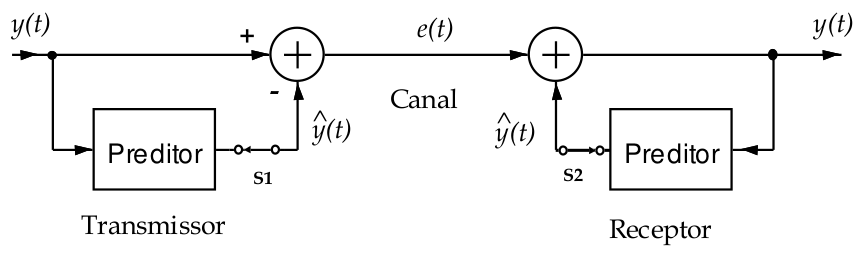
\includegraphics[height=4cm]{figPreditor.png}
	\end{center}
	\legend{Fonte: ver referência \cite{tvDigitalUSP}.}
\end{figure}

Para a predição de sinais de video, é necessário realizar uma compensação de movimento, ou seja, uma estimação do movimento dos objetos presentes em quadros subsequentes. O movimento é descrito como um vetor de movimento bidimensional com o tamanho e direção igual ao do movimento. A \autoref{figMV} apresenta os vetores de movimento, onde a segunda imagem pode ser reconstruída a partir da primeira usando os vetores de movimento. A implementação estimação do movimento é eficiente quando o brilho dos objetos é constante ao longo do tempo e pontos de um quadro próximos tendem a apresentar o mesmo movimento \cite{ogeMatlab} \cite{tvDigitalUSP}.

\begin{figure}[htb]
	\caption{\label{figMV} Dois quandros representando o mesmo objeto em instantes de tempo diferentes e o fluxo de movimento.}
	\begin{center}
		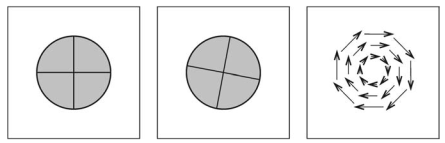
\includegraphics[height=4cm]{figMV.png}
	\end{center}
	\legend{Fonte: ver referência \cite{ogeMatlab}.}
\end{figure}

Sendo impossível detectar todos objetos reais presentes na imagem dentro de um tempo de compressão, a imagem é segmenta em vários blocos, onde o vetor movimento tem a função de informar o deslocamento que este bloco no próximo quadro. O detector de movimento percorre a imagem buscando o ponto de menor diferença com o bloco de referencia. Esta diferença e dada pela distorção media absoluta, com equacionamento sendo
\begin{equation}
DMA(x,y)\ddfrac{1}{N}\sum_{i,j}\left|f\left(x+i,y+j\right)-ref\left(x+i+dx,y+j+dy\right)\right|
\end{equation}
onde, $(dx,dy)$ é o deslocamento entre a imagem de referência $ref(x,y)$. Quando $DMA$ é mínimo, $(dx,dy)$ é o vetor de movimento para o bloco em $(x,y)$. A \autoref{figEstimador} apresenta graficamente esta operação \cite{tvDigitalUSP}.

\begin{figure}[htb]
	\caption{\label{figEstimador} Estimador de Movimento.}
	\begin{center}
		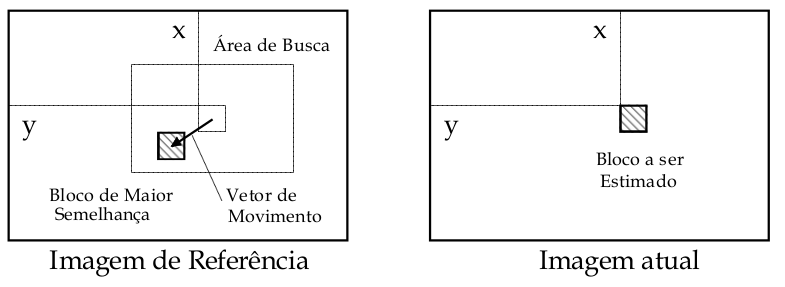
\includegraphics[height=4cm]{figEstimador.png}
	\end{center}
	\legend{Fonte: ver referência \cite{tvDigitalUSP}.}
\end{figure}

%\section{Transformada discreta de cossenos}
%O que é e para que serve a transformada discreta de cossenos.


\section{Compressão MPEG-1}
%Como funciona o padrão de compressão MPEG-1e quais são as etapas de processamento.

\textit{Moving Pictures Experts Group} é um padrão de compressão de imagens em movimentos para vídeo-CD (CD-ROM), com sinal de áudio operando em taxas de 192 kbps e vídeo em 1,15 Mbps, com a imagem no formato 320x240 pixels \cite{oge}. As taxas de compressão com perdas podem ser maiores que 50:1 

%\section{Estrutura dos quadros MPEG}
%Como funciona a estrutura dos quadros MPEG e a interdependência entre eles.


Os quadros do vídeo são classificados em três tipos: I (\textit{intraframe}) P (preditivo) e B (bidirecional). A compressão do quadro I é realizada de forma similar ao padrão JPEG, não se utilizando de outros quadros, por isso é considerado a referência temporal e apresenta taxa de compressão baixa em relação aos outros. O quadro P apresenta compressão com predição por um I ou P anterior, a compressão do quadro P é maior que a do I. Por ultimo, o quadro B, que apresenta maior compressão entre todos, usa como referencia dois quadros, um anterior e outro posterior do tipo I ou P \cite{oge}.


Grupos de Imagens (\textit{GOP's - Groups of Pictures}),  é uma sequencia de quadros  do tipo I, P e B, \autoref{figIPB} em várias proporções, onde todas as operações utilizam somente os quadros dentro do GOP. Na \autoref{figIPB} a distância entre imagens tipo I ($M$) é 9 e entre imagens P ($N$) é 3. Os quadros  I e P são transmitidos  primeiros, pois serão utilizados para reconstruir os quadros B intermediarias \cite{tvDigitalUSP}. Os quadros I garantem a qualidade de GOP, pois os quadros P e B são baseados nele. Os quadros B consome pouca largura de banda e torna o GOP mais suave, porém implica na necessidade de armazenamento de quadros P, aumentando o custo computacional \cite{oge}.

\begin{figure}[htb]
	\caption{\label{figIPB} Grupos de Imagens em MPEG-1.}
	\begin{center}
		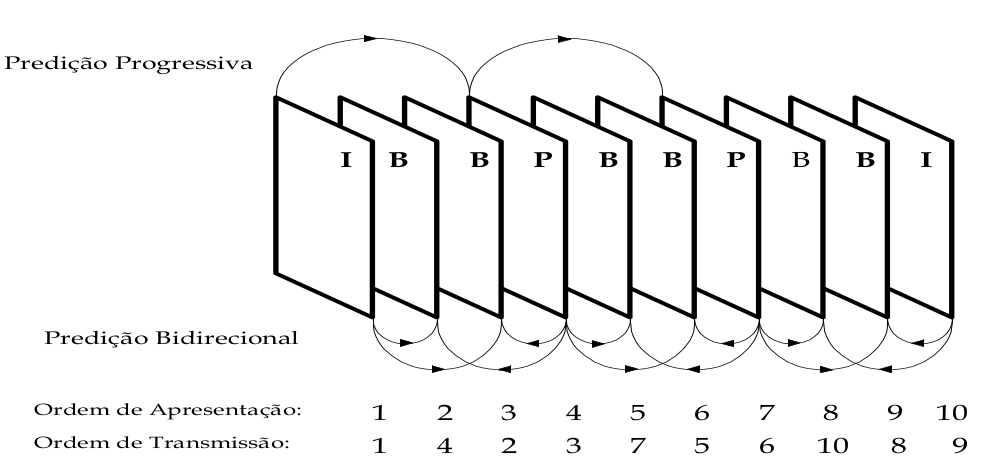
\includegraphics[height=4cm]{figIPB.png}
	\end{center}
	\legend{Fonte: ver referência \cite{tvDigitalUSP}.}
\end{figure}

A \autoref{figMPEG} apresenta o algoritmo do codificador MPEG-1. O bloco, ou imagem, é a entrada, o classificador formatador formata a imagem para 320x240 pixels de luminância e 160x120 pixels de componentes de crominância (amostragem 4:2:0), em sequência estes dois planos são divididos em blocos 8x8 pixels. O preditor de detecção de movimento agrupa os blocos em macroblocos (4 blocos 8x8) e gera os vetores de movimento transmitidos diretamente ao receptor (saída). O preditor, ainda, realiza uma estimativa, baseando-se nas imagens de referencia, e transmite os blocos estimados. É calculada a diferença dos blocos originais e os estimados. Sobre este sinal erro, é aplicada a  transformada discreta de cossenos (DCT), tendo a função de eliminar de redundâncias espacias da imagem erro. A resposta da DCT  é quantizada  por valores de tabelados pela padrão JPEG. Os coeficientes gerados pela quantização são compactos seguindo o processo de compressão JPEG, onde é utilizado a codificação RLE (\textit{Run-Length Encoding}) para gerar
um símbolo para cada coeficiente. Este símbolo é um par
ordenado de dois números, sendo o primeiro quantidade de zeros antes do coeficiente e o próprio valor do coeficiente. Posteriormente é aplicado a codificação de Huffman, sendo gerado novo símbolo contendo as informações da quantidade de zeros, a quantidade de bits para representar o valor do coeficiente \cite{tvDigitalUSP}.


A etapas inversas da quantização e da DCT são realizadas para gerar as imagens de referencia quando os quadros de entrada forem P ou I \cite{tvDigitalUSP}.  

\begin{figure}[htb]
	\caption{\label{figMPEG} Codificador MPEG-1.}
	\begin{center}
		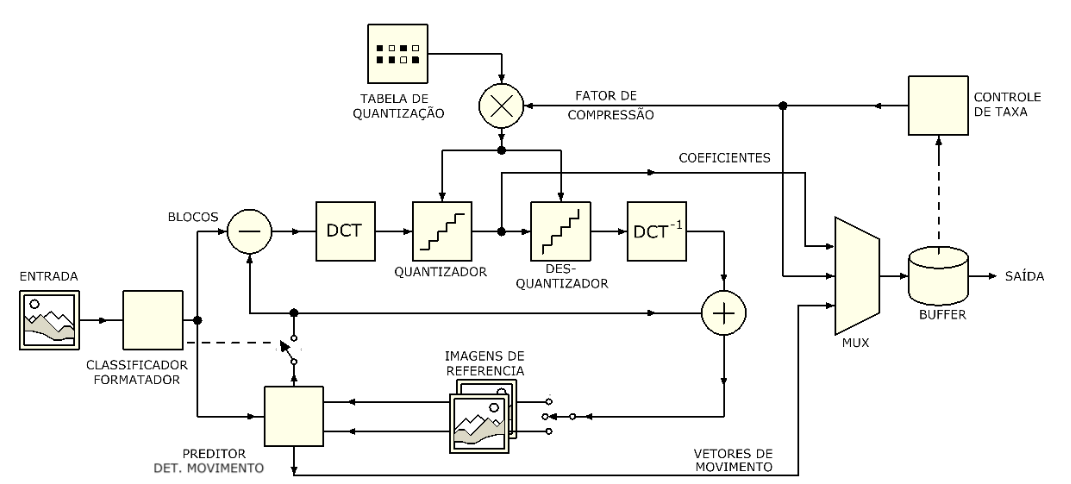
\includegraphics[width=\ScaleIfNeeded]{figMPEG.png}
	\end{center}
	\legend{Fonte: ver referência \cite{tvDigitalUSP}.}
\end{figure}


A descompressão do video MPEG-1, \autoref{figDeMPEG}, inicia obtendo as informações do fator de compressão, os vetores de movimento e os símbolos da codificação de Huffman. Os quadros P e I estão no inicio da fila de transmissão, são decodificados e os vetores de movimento os utilizam para prever os quadros B \cite{tvDigitalUSP}.

\begin{figure}[htb]
	\caption{\label{figDeMPEG} Decodificador MPEG-1.}
	\begin{center}
		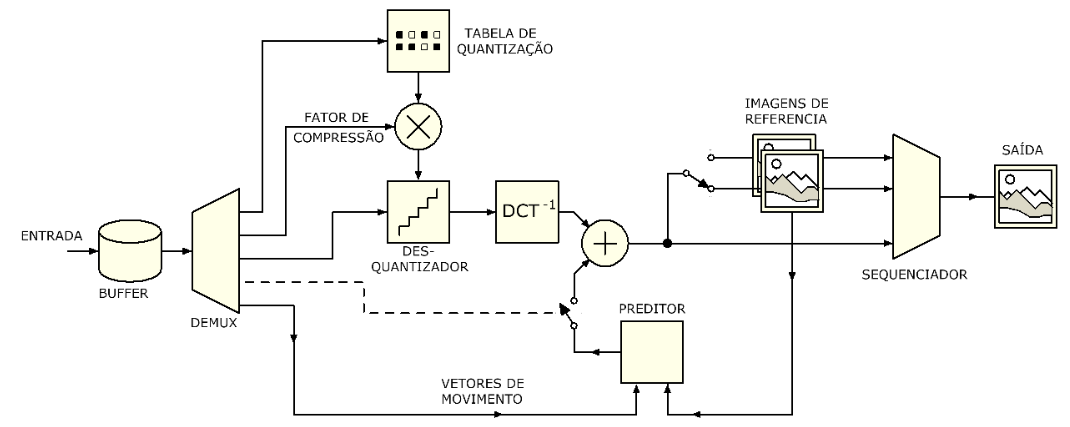
\includegraphics[width=\ScaleIfNeeded]{figDeMPEG.png}
	\end{center}
	\legend{Fonte: ver referência \cite{tvDigitalUSP}.}
\end{figure}

\section{Compressão do áudio}

O áudio de uma televisão digital deve possibilitar a melhor experiencia ao telespectador. Para isso, deve-se transmitir 5 canais principais (direito, esquerdo, central, traseiro esquerdo e traseiro direito) com frequência de amostragem 48 kHz e quantização nativa de 24 bits. Neste caso a taxa seria de 5,88 MB/s, representado 1/4 da capacidade de uma canal para TV digital. Assim, a compressão se torna indispensável \cite{tvDigitalUSP}. 

A compressão de áudio é baseada no  efeito máscara, estando relacionado com a percepção dos sons pelo ouvido humano em relação a suas frequências. Dado um som, ou tom, sendoidal em uma frequência de maior amplitude, o ouvido reduz sua sensibilidade para outros sons em frequências próximas em até 20 dB. Quanto maior a amplitude do tom, maior o alcance de atenuação. O ouvido também gera atenuações para as frequências harmônicas do tom de grande amplitude.
Desta forma, na codificação do sinal de áudio, é possível eliminar frequência dentro da banda de atenuação de sons altos, pois o ouvido humano não irá perceber estes sons. Assim, é reduzida a quantidade de informação do arquivo de som sem prejudicar a sua qualidade.


O codificador de áudio, \autoref{figCodAudio}, utiliza-se de filtros conhecidos por QMF (Quadrature Mirror Filters) para decompor o sinal em sub-bandas, provavelmente relacionadas às bandas críticas de audibilidade. As sub-bandas passam por um processo gerando uma banda estreita. É realizada a estimativa do do mascaramento para calcular a relação sinal ruído necessário, é realizada a quantização e gerando, finalmente, o fluxo de dados codificados do sinal de áudio. 

\begin{figure}[htb]
	\caption{\label{figCodAudio} Estrutura do Codificador MPEG-Áudio.}
	\begin{center}
		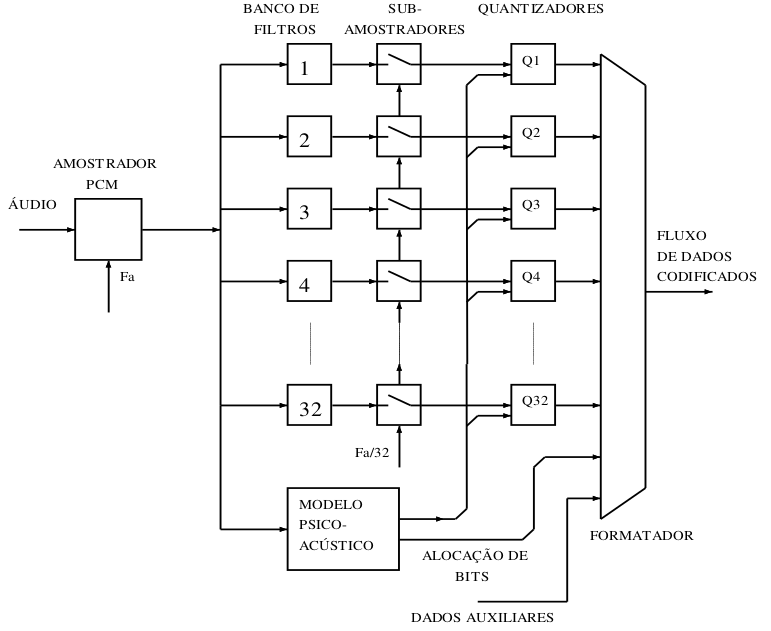
\includegraphics[width=\ScaleIfNeeded]{figCodAudio.png}
	\end{center}
	\legend{Fonte: ver referência \cite{tvDigitalUSP}.}
\end{figure}
% ----------------------------------------------------------

% ------------------------------------------------
% Referências bibliográficas
%\makeatletter
%\renewcommand\@biblabel[1]{{\parbox{0.8cm}{[#1]}}}
%\makeatother
%\bibliography{tex_latexReferencias}
\printbibliography
% ------------------------------------------------

\end{document}
